\documentclass{article}
\usepackage[utf8]{inputenc}
\usepackage{multicol}
\usepackage[formats]{listings}
\lstloadaspects{formats}
\usepackage{verbatim}
\usepackage{color}
\usepackage{geometry}
\usepackage{float}
\usepackage{amsmath}
\usepackage{caption}
\usepackage{pdflscape}

\usepackage{hyperref}
\setlength{\belowcaptionskip}{-10pt}
\setlength{\abovecaptionskip}{-30pt}
\floatstyle{boxed} 
\restylefloat{figure}
\usepackage{graphicx}
\definecolor{codegreen}{rgb}{0,0.6,0}
\definecolor{codegray}{rgb}{0.5,0.5,0.5}
\definecolor{codepurple}{rgb}{0.58,0,0.82}
\definecolor{backcolour}{rgb}{0.95,0.95,0.92}
\lstdefinestyle{mystyle}{
	backgroundcolor=\color{backcolour},   
	commentstyle=\color{codegreen},
	keywordstyle=\color{blue},
	numberstyle=\tiny\color{codegray},
	stringstyle=\color{codepurple},
	basicstyle=\footnotesize,
	breakatwhitespace=false,         
	breaklines=true,                 
	captionpos=b,                    
	keepspaces=true,                 
	numbers=left,                    
	numbersep=5pt,                  
	showspaces=false,                
	showstringspaces=false,
	showtabs=false,                  
	tabsize=2
}
\lstset{style=mystyle}
\title{Data Mining\\
		Home work 10\\Machine Learning III Regression Analysis }
\author{Aqeel Labash\\ \textbf{Lecturer:} Jaak Vilo}
\date{13 April 2016}
\geometry{
	a4paper,
	total={170mm,257mm},	
	left=10mm,
	top=5mm,
}
\begin{document}
	\maketitle
\section*{First Question}
For this task I used python and here is the code : 
\begin{lstlisting}[language=Python]
# #Question 1
import numpy as np
get_ipython().magic(u'matplotlib inline')
import matplotlib.pyplot as plt
points = [(9,3,1),(2,4,1),(3,3,1),(4,1,1),(1,6,1),(3,9,0),(5,6,0),(6,4,0),(6,2,0),(3,7,0)]
#Draw the figure
plt.figure('points.jpg')
plt.plot([x[0] for x in points],[x[1] for x in points],'bo')
plt.plot([3,4],[5,6],'rv')
plt.ylabel('Y')
plt.xlabel('X')
plt.title('Points')
plt.savefig('points.jpg')

#Print Probabilities for classes
def GetClosePoints(centerpoint,k=1):
    indx =0
    distances={}
    for point in points:
        
        #Calculate Eucludean distance
        distance = np.linalg.norm(np.array(centerpoint)-np.array((point[0],point[1])))
        
        #Store all points with the same distance under the same 
        if distance in distances.keys():
            distances[distance].append(indx)
        else:
            distances[distance] = []
            distances[distance].append(indx)
        indx+=1
        
    #Sort list by distance
    keys = distances.keys()
    keys.sort(key = lambda x:x,reverse=False)
    #print the list 
    #for key in keys:
    #    print key , distances[key]
        
    #Get Points in K distance
    pointindx=[]
    for i in range (0,k):
        for index in distances[keys[i]]:
            pointindx.append(index)

    #Print Selected Points indexs 
    #print pointindx
    
    #Calculate Probabilities
    Totalpoints = len(pointindx)
    Class0=0
    Class1=0
    for i in pointindx:
        if points[i][2]:
            Class1+=1
        else:
            Class0+=1
    print 'For Point ({},{}) with K={},Probabilities is Class 0:{},Class 1:{}'.format(centerpoint[0],centerpoint[1],k,
    Class0/float(Totalpoints),Class1/float(Totalpoints))
p1 = (3,5)
p2 = (4,6)
GetClosePoints(p1,1)
GetClosePoints(p1,2)
GetClosePoints(p1,3)
GetClosePoints(p2,1)
GetClosePoints(p2,2)
GetClosePoints(p2,3)
\end{lstlisting}
What  I did in the previous code is:
\begin{enumerate}
	\item Store the indexes of points with same distance from our point under same hash label.
	\item Select the indexes depending on K
	\item Count total points,points in class0 , points in class1
	\item Print the probabilities
\end{enumerate}
Here is an image showing how the points look like :
\begin{figure}[H]
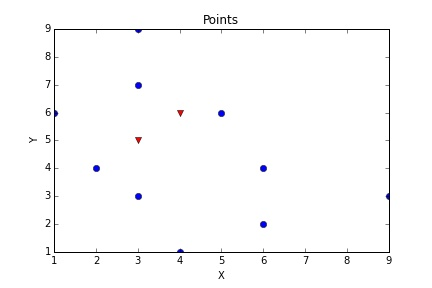
\includegraphics[scale=1]{points.jpg}
\caption{Points in the plane.}
\end{figure}
And here I report the output of the previous code :\\
For Point (3,5) with K=1,Probabilities is Class0=0.0,Class1=1.0\\
For Point (3,5) with K=2,Probabilities is Class0=0.333333333333,Class1=0.666666666667\\
For Point (3,5) with K=3,Probabilities is Class0=0.4,Class1=0.6\\
For Point (4,6) with K=1,Probabilities is Class0=1.0,Class1=0.0\\
For Point (4,6) with K=2,Probabilities is Class0=1.0,Class1=0.0\\
For Point (4,6) with K=3,Probabilities is Class0=0.75,Class1=0.25
\section*{Second Question}
For this question I build my own function to calculate the measurements from confusion matrix , here is the code:
\begin{lstlisting}[language=R]
measuresprint<-function(cm)
{
  Accuracy<-(cm[2,2]+cm[1,1])/sum(cm)
  Precision<-(cm[2,2])/(cm[2,2]+cm[1,2])
  Recall<-cm[2,2]/(cm[2,2]+cm[2,1])
  F1<-2*(Precision*Recall)/(Precision+Recall)
  print(c(Accuracy,Precision,Recall,F1))
}
###### Second Question ########
diabetes <- read.csv('pima-indians-diabetes.data',header = FALSE)
colnames(diabetes)<-c('PregnantTimes','glucos_constr','Blood_pressure','Triceps','insulin','BMI','diabts_pedigree','Age','Class')
#Shuffle The list so we pick randomly 
diabetes<- diabetes[sample(nrow(diabetes)),]
traindata<-diabetes[seq(1,floor(nrow(diabetes)*0.8),1),]
test<-diabetes[seq(floor(nrow(diabetes)*0.8)+1,nrow(diabetes)),]
module <- glm(Class~.,data = traindata)
summary(module)
png('correlationhm.png')
heatmap(cor(diabetes),symm = TRUE, Colv=NA, Rowv=NA,col=colorRampPalette(c("red", "yellow", "green"))(n = 299))
dev.off()

#prediction_prop<-
prediction_bin<-ifelse(predict(module, test)<=0.5,0,1)
measuresprint(table(real=test$Class, predictions=prediction_bin))
\end{lstlisting}
The summary of the module output was :
\begin{lstlisting}
Coefficients:
                  Estimate Std. Error t value Pr(>|t|)    
(Intercept)     -0.8270580  0.0952931  -8.679  < 2e-16 ***
PregnantTimes    0.0227378  0.0055950   4.064 5.46e-05 ***
glucos_constr    0.0058791  0.0005769  10.192  < 2e-16 ***
Blood_pressure  -0.0027814  0.0009006  -3.088  0.00211 ** 
Triceps         -0.0001970  0.0012530  -0.157  0.87511    
insulin         -0.0002141  0.0001702  -1.258  0.20893    
BMI              0.0135468  0.0022537   6.011 3.19e-09 ***
diabts_pedigree  0.1493781  0.0511308   2.921  0.00361 ** 
Age              0.0024483  0.0017115   1.430  0.15310    
---
\end{lstlisting}
From the summary we can notice that "Plasma glucose concentration" which equals to "glucos\_constr" in table , that it's high significant to predict the class. Also we can see that it's highly correlated with the class.
\begin{figure}[H]
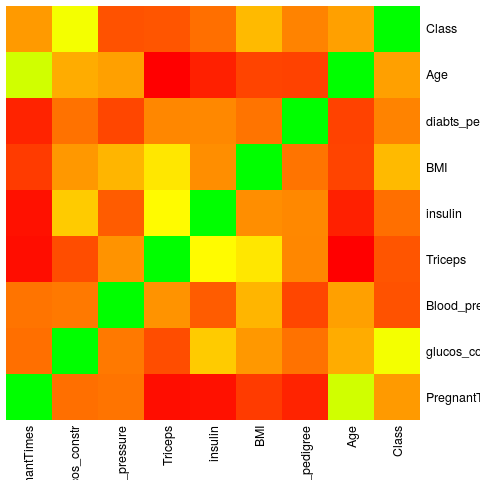
\includegraphics[scale=0.9]{correlationhm.png}
\caption{Heatmap for correlation}
\end{figure}
From the previous figure we can see that plasma glucos is the most correlated to the class.\\
For "diabetes pedigree" we can see from the table that it's 2 stars significant, and from the correlation picture we can see it's less correlated than plasma glucos.\\
To do the calcuation I printed out the confusion matrix \\
\begin{tabular}{|c|c|c|}
\hline
real\_ predic&0&1\\ \hline
0& 84 & 15 \\ \hline
   1 &22 &33\\ \hline
\end{tabular}
The rules for the measurements :
\[Accuracy = \frac{TP+TN}{Total} \]
\[Precision = \frac{TP}{TP+FP}\]
\[Recall = \frac{TP}{TP+FN} \]
F1 "is the harmonic mean of precision and sensitivity" \cite{1}
\[F1 =\frac{2TP}{2TP+FP+FN}\]
Another way to calculate it
\[F1 =2.\frac{precision*recall}{precision+recall}\]
The measurements :\[ Accuracy=0.7597403,Precision= 0.6875000,Recall= 0.6000000,F1= 0.6407767\]
\section*{Third Question}
For this question I used the function knn in R and here is the code : 
\begin{lstlisting}[language=R]
####### Third Question#####
library(class)
knn1prediction<-knn(traindata,test = test,cl=traindata$Class)
measuresprint(table(real=test$Class, predictions=knn1prediction))
knn3prediction<-knn(traindata,test = test,cl=traindata$Class,k = 3)
measuresprint(table(real=test$Class, predictions=knn3prediction))
\end{lstlisting}
From the previous code we get the measurements for k1 and k3 and in the following table I put all the measurements for k1,k3 and glm to compare them\\
\begin{tabular}{|l|*{5}{c|}}
\hline
Method&Accuracy&Precision&Recall&F1\\ \hline
glm&0.7597403&0.6875000&0.6000000&0.6407767\\ \hline
K1&0.6948052&0.5769231&0.5454545&0.5607477\\ \hline
K3&0.7272727&0.6181818&0.6181818&0.6181818\\ \hline
\end{tabular}\\
From the previous table we can see that logit regression got the best Accuracy and the highest F1 score.
\section*{Fourth Question}
For this question I used the following code : 
\begin{lstlisting}[language=R]
########## Fourth Question ###########
rm(list=ls())
setwd('/home/aqeel/Study/DM/HW10/')
library(ggplot2)
data("diamonds")
diamonds<- diamonds[sample(nrow(diamonds)),]
trainset<-diamonds[seq(1,floor(0.8*nrow(diamonds))),]
testset<-diamonds[seq(floor(0.8*nrow(diamonds))+1,nrow(diamonds)),]
module1<-lm(price~.,data = trainset)
module2<-lm(price~.+poly(carat,2)+poly(depth,2)-carat-depth,data = trainset)
module3<-lm(price~.+poly(carat,3)+poly(depth,3)-carat-depth,data = trainset)
module4<-lm(price~.+poly(carat,3)+poly(depth,3)+poly(x,2)+poly(y,2)+poly(z,2)-carat-depth-x-y-z,data = trainset)
module1predtrn<-predict(module1, trainset)
module2predtrn<-predict(module2, trainset)
module3predtrn<-predict(module3, trainset)
module4predtrn<-predict(module4, trainset)
module1predtst<-predict(module1, testset)
module2predtst<-predict(module2, testset)
module3predtst<-predict(module3, testset)
module4predtst<-predict(module4, testset)
#install.packages("qpcR")
library(qpcR)
trainRMSE<-c(sqrt(sum((module1predtrn-trainset$price)^2)/length(trainset$price)),
sqrt(sum((module2predtrn-trainset$price)^2)/length(trainset$price)),
sqrt(sum((module3predtrn-trainset$price)^2)/length(trainset$price)),
sqrt(sum((module4predtrn-trainset$price)^2)/length(trainset$price)))

testRMSE<-c(sqrt(sum((module1predtst-testset$price)^2)/length(testset$price)),
sqrt(sum((module2predtst-testset$price)^2)/length(testset$price)),
sqrt(sum((module3predtst-testset$price)^2)/length(testset$price)),
sqrt(sum((module4predtst-testset$price)^2)/length(testset$price)))
numbers<-seq(1,4,1)
png('train_test.png')
ggplot(data.frame(cbind(numbers,trainRMSE)),aes(numbers, trainRMSE))+geom_line(col="red") +
  geom_line(aes(numbers,testRMSE),data =data.frame(cbind(numbers,testRMSE)),col="blue" )+ xlab("Module")+
  ylab("RSME")
\end{lstlisting}

The previous code will output the following picture which represent the Train vs Test RMSE value.
\begin{figure}[H]
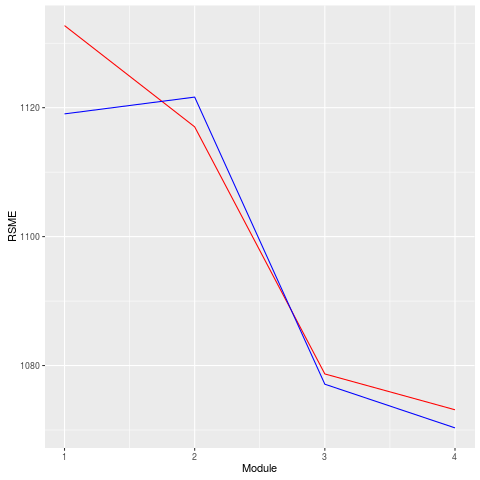
\includegraphics[scale=1]{train_test.png}
\caption{Train RMSE in Red , Test in blue}
\end{figure}
I would detect overfiting when the training RMSE keep decreasing while the testing RMSE start increasing. I believe we can see that from the plot after doing many iteration for the same module.With only one iteration it's hard to decide if we have overfiting mmmm maybe we can if the RMSE was pretty low for training and pretty high for testing.\\
Also I would notice from the plot that module 4 performed the best :).
\section*{Fifth Question}
For this question I used straight forward solution and here is the code :
\begin{lstlisting}[language=R]
rm(list=ls())
setwd('/home/aqeel/Study/DM/HW10/')
train <- read.csv('train.csv',header = TRUE)
module<-lm(data = train,target~.)
summary(train)
test<-read.csv('test.csv',header = TRUE)
head(test[,c(1,2)])
result<-predict(module,test)
output<-cbind(result)
colnames(output)<-c('ID','target')

write.csv(output,file='submit 001')
\end{lstlisting}
I got  	score 1.95523 for this code :) 





\section*{Sixth Question}
\section*{Seventh Question} 

The code for this question :
\begin{lstlisting}[language=R]
################ Seventh Question ############
library(MASS)
module4ridge<- lm.ridge(price~.+poly(carat,3)+poly(depth,3)+poly(x,2)+poly(y,2)+poly(z,2)-carat-depth-x-y-z,data = trainset)
module4ridge.trn.prd = as.matrix(model.matrix(price~.+poly(carat,3)+poly(depth,3)+poly(x,2)+poly(y,2)+poly(z,2)-carat-depth-x-y-z,trainset))%*% coef(module4ridge)
module4ridge.tst.prd = as.matrix(model.matrix(price~.+poly(carat,3)+poly(depth,3)+poly(x,2)+poly(y,2)+poly(z,2)-carat-depth-x-y-z,testset))%*% coef(module4ridge)


#install.packages("lars")
library(lars)
module4lasso <- lars(
  model.matrix(price~.+poly(carat,3)+poly(depth,3)+poly(x,2)+poly(y,2)+poly(z,2)-carat-depth-x-y-z,trainset),
  trainset$price, type="lasso",trace = TRUE, max.steps=20)
module4lasso.trn.prd <- predict(module4lasso,
                        model.matrix(price~.+poly(carat,3)+poly(depth,3)+poly(x,2)+poly(y,2)+poly(z,2)-carat-depth-x-y-z,trainset),
                        s=module4lasso$df[which.min(module4lasso$RSS)], type="fit")$fit


module4lasso.tst.prd <- predict(module4lasso,
                                model.matrix(price~.+poly(carat,3)+poly(depth,3)+poly(x,2)+poly(y,2)+poly(z,2)-carat-depth-x-y-z,testset),
                                s=module4lasso$df[which.min(module4lasso$RSS)], type="fit")$fit

trainRMSE<-c(sqrt(sum((module1predtrn-trainset$price)^2)/length(trainset$price)),
             sqrt(sum((module2predtrn-trainset$price)^2)/length(trainset$price)),
             sqrt(sum((module3predtrn-trainset$price)^2)/length(trainset$price)),
             sqrt(sum((module4predtrn-trainset$price)^2)/length(trainset$price)),
             sqrt(sum(( module4lasso.trn.prd- trainset$price)^2)/length(trainset$price)),
             sqrt(sum((module4ridge.trn.prd- trainset$price)^2)/length(trainset$price)))

testRMSE<-c(sqrt(sum((module1predtst-testset$price)^2)/length(testset$price)),
            sqrt(sum((module2predtst-testset$price)^2)/length(testset$price)),
            sqrt(sum((module3predtst-testset$price)^2)/length(testset$price)),
            sqrt(sum((module4predtst-testset$price)^2)/length(testset$price)),
            sqrt(sum(( module4lasso.tst.prd- testset$price)^2)/length(testset$price)),
            sqrt(sum((module4ridge.tst.prd- testset$price)^2)/length(testset$price)))
numbers<-seq(1,6,1)
png('all_modules.png')
ggplot(data.frame(cbind(numbers,trainRMSE)),aes(numbers, trainRMSE))+geom_line(col="red") +
  geom_line(aes(numbers,testRMSE),data =data.frame(cbind(numbers,testRMSE)),col="blue" )+ xlab("Module")+
  ylab("RSME")
dev.off()
\end{lstlisting}
The RMSE for lasso and ridge was quite high so it won't be much clear in the graph but here is the graph : \\
\begin{figure}[H]
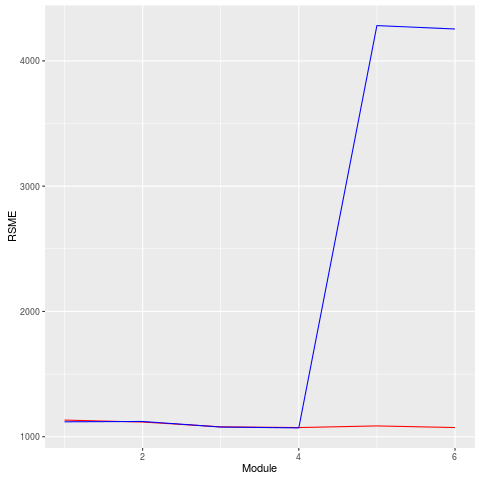
\includegraphics[scale=1]{all_modules.png}
\caption{Last two values are lasso and ridge}
\end{figure}
\textbf{Please note:}Faiz helped a lot in this question.
\begin{thebibliography}{9}
	\bibitem{1}
	\href{https://en.wikipedia.org/wiki/Precision_and_recall}{Precision and Recall}
\end{thebibliography}
\end{document}